\documentclass{subfiles}
\begin{document}
\begin{figure}[!h]
    \centering
    \begin{subfigure}[b]{0.425\textwidth}
        \centering
        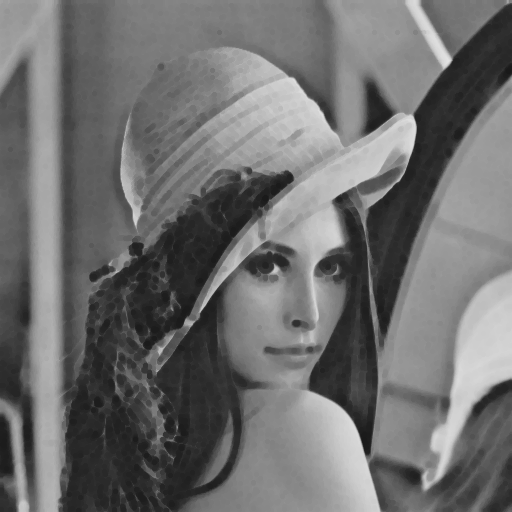
\includegraphics[scale = 0.325]{../Images/Lena/Eroded Lena.png}
        \caption{\(\varepsilon_{S}(I)\).}
    \end{subfigure}
    \hspace{10pt}
    \begin{subfigure}[b]{0.425\textwidth}
        \centering
        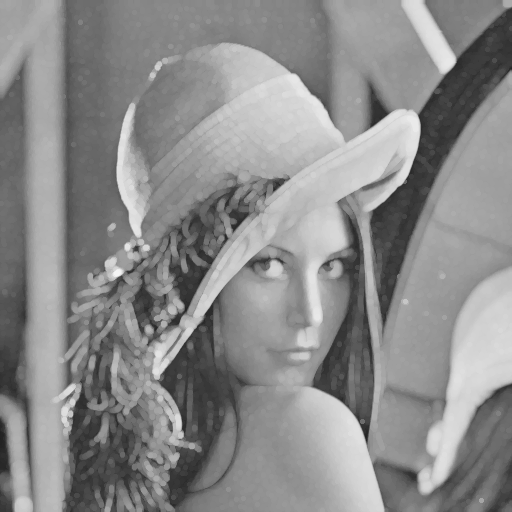
\includegraphics[scale = 0.325]{../Images/Lena/Dilated Lena.png}
        \caption{\(\delta_{S}(I)\).}
    \end{subfigure}
    \caption{Applicazione delle operazioni di erosione e dilatazione a \emph{Figura \ref{fig:4.1}}.}
    \label{fig:7.1}
\end{figure}
\end{document}